% Drawing 80/04-1 -- folder 80, batch 04, archive page 63 (PDF page 64).
% Transcription: à gauche, un dessin au crayon : deux droites $D$ et $D'$ issues d'un point $t$ (à gauche), une droite verticale $\Delta$ passant par $s$ (en bas), une droite $\Delta'$ issue de $s$ vers la gauche, une droite horizontale épaissie $\Gamma'$ et une droite oblique $\Gamma$ (en haut) ; les points $u$ (sur $D$) et $u'$ (sur $D'$) sont marqués sur la verticale
% Kind: pencil drawing of lines. Method 2 (schematic redraw from the facsimile). Status: partial.
% Notes: Faint pencil: the two lines D, D' from t (left), the vertical Delta through s (bottom), Delta' from s to the left, the horizontal Gamma' thickened in its middle, the oblique Gamma at the top; u and u' marked on the vertical. The labels D, D', Gamma, Gamma' are not legible on the crop and are left out; which line is which follows the transcription.
% Coordinates: 1 unit = 1 mm = 1/100 of the crop width (bbox in page fractions: [0.08, 0.52, 0.38, 0.72]).
% Redrawn by Claude (claude-opus-5-5), issue #73, 2026-11-07; not checked by a human; not compiled (no TeX in the session).
% Rights: reproduces part of the work -- behind RENDER_TRANSCRIPTS, never published by itself.
\documentclass[tikz,border=3pt]{standalone}
\usepackage{amsmath,amssymb}
\usetikzlibrary{patterns,arrows.meta}
\tikzset{pencil/.style={black!45}, struck/.style={black!35}, mark/.style={circle,draw,inner sep=1.3pt}, pt/.style={circle,fill,inner sep=0.9pt}, opt/.style={circle,draw,fill=white,inner sep=1.1pt}}
\begin{document}
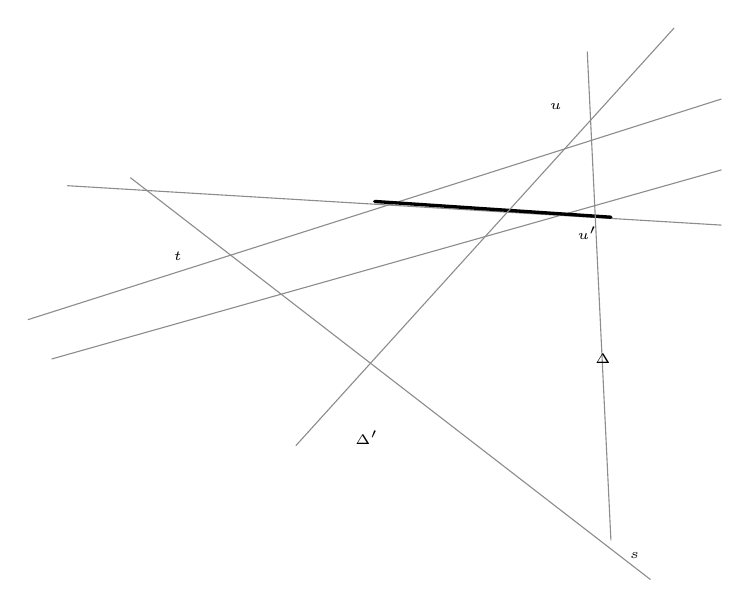
\begin{tikzpicture}[x=1mm,y=1mm,line cap=round,line join=round,font=\scriptsize]
\draw[pencil] (6,-52) -- (94,-24);
\draw[pencil] (9,-57) -- (94,-33);
\draw[pencil] (11,-35) -- (94,-40);
\draw[very thick] (50,-37) -- (80,-39);
\draw[pencil] (40,-68) -- (88,-15);
\draw[pencil] (77,-18) -- (80,-80);
\draw[pencil] (19,-34) -- (85,-85);
\node[inner sep=1pt] at (25,-44) {\tiny $t$};
\node[inner sep=1pt] at (73,-25) {\tiny $u$};
\node[inner sep=1pt] at (77,-41) {\tiny $u'$};
\node[inner sep=1pt] at (79,-57) {\tiny $\Delta$};
\node[inner sep=1pt] at (49,-67) {\tiny $\Delta'$};
\node[inner sep=1pt] at (83,-82) {\tiny $s$};
\end{tikzpicture}
\end{document}
